\newpage
\section{Preliminaries}
\label{sec:prelim}

For the interested reader, in this section we introduce the basic definitions and notions that are used
in the forthcoming sections of this work, we also introduce the basic notation that we are going to use.

\subsection{Graph Databases}

\subsubsection*{Graph Data Model: Property Graph}\label{prelim:graphdatamodel-pg}

% 1. Graph DATA model
A data[base] model is a collection of conceptual tools used to model representations of real-world entities and the relationships among them \cite{GDB-angles2008survey}. A graph database model is a data[base] model for the understanding and management of graph data \cite{GDB-kumar2015graph}. There are three dominant graph data models: the property graph, Resource Description Framework (RDF) triples, and hypergraphs. A commonly employed graph data model in practice is the property graph data model \cite{Graph-Databases-OReally-book, PG-angles2017foundations}. This will be our selected graph database model.\\

Informally, a property graph (PG) is a directed labeled multigraph with the special characteristic that each node or edge could maintain a set (possibly empty) of property-value pairs. In this graph, a node represents an entity, an edge a relationship between entities, and a property represents a specific feature of an entity or relationship. More formally, we provide the same definition as the one in \cite{angles2018propertyGraphDatabaseModel}:

\begin{definition}
A property graph is a tuple $G=(N,E, \rho, \lambda, \sigma)$ where:
\begin{enumerate}
    \item $N$ is a finite set of nodes (also called vertices);
    \item $E$ is a finite set of edges such that $E$ has no elements in common with $N$;
    \item $\rho: E \rightarrow (N \times N)$ is a total function that associates each edge in $E$ with a pair of nodes in $N$ (i.e., $\rho$ is the usual incidence function in graph theory);
    \item $\lambda: (N \cup E) \rightarrow SET^{+}(\textbf{L})$ is a partial function that associates a node/edge with a set of labels from $L$ (i.e., $\lambda$ is a labeling function for nodes and edges);
    \item $\sigma: (N \cup E) \times \textbf{P} \rightarrow SET^{+}(V)$ is a partial function that associates nodes/edges with properties, and for each property it assigns a set of values from $\textbf{V}$.
\end{enumerate}
Where $\textbf{L}$ is an infinite set of labels (for nodes and edges), $\textbf{P}$ is an
infinite set of property names, $\textbf{V}$ is an infinite set of atomic values, and $\textbf{T}$ is a finite set of datatypes (e.g., integer). Given a set $X$, we assume that $SET^{+}(X)$ is the set of all finite subsets of $X$, excluding the empty set. Given a value $v \in \textbf{V}$, the function type($v$) returns the data type of $v$. The values in $\textbf{V}$ will be distinguished as quoted strings.
\end{definition}

Given two nodes $n_1$, $n_2$ $\in N$ and an edge $e \in E$, such that $\rho(e) = (n_1, n_2)$,
we will say that $n_1$ and $n_2$ are the “source node” and the “target node” of
$e$ respectively. Additionally, given a property $(o, p) \in (N \cup E) \times \textbf{P}$ and the
assignment $\sigma(o, p) = \{v_1,...,v_n\}$, we will use $(o, p) = v_i$ with $1 \leq i \leq n$ as a shorthand representation for a single property where $o$ is the “property owner”,
$p$ is the “property name” and $v$ is the “property value”. Note that their definition
supports multiple labels for nodes and edges, and multiple values for the same
property.

\begin{figure}[H]
    \centering
    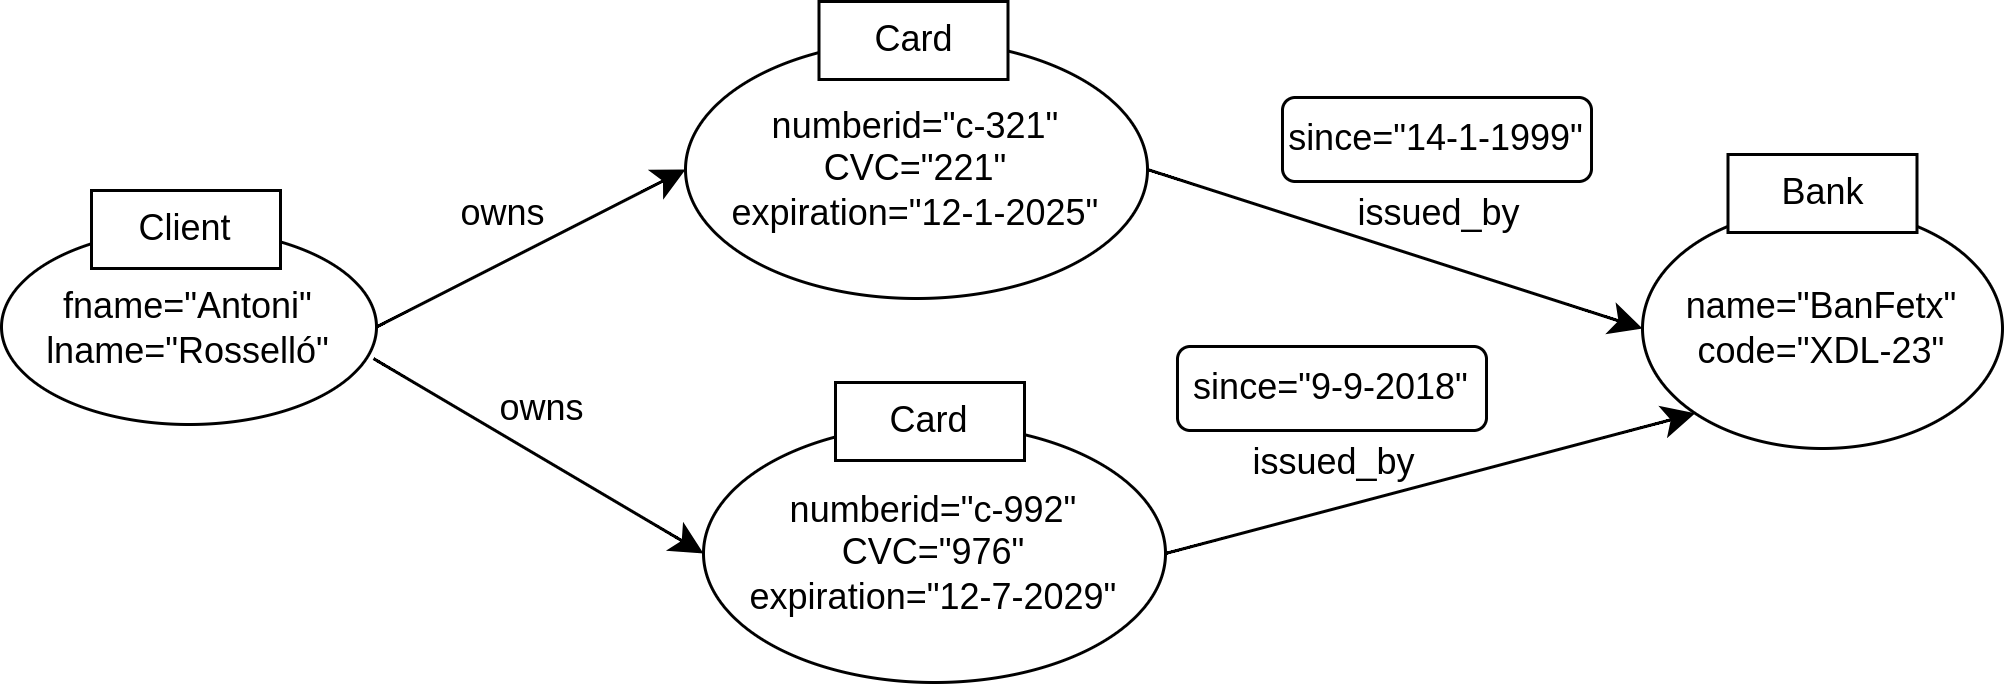
\includegraphics[scale=0.8]{images/PG-DEF.png}
    \caption{Property graph example representing bank database information}
    \label{img:PG-example}
\end{figure}

As an example we provide Figure \ref{img:PG-example}, where we show a property graph representing bank data information. With respect to the formal definition given we have:
\begin{itemize}
    \item $N = \{n_1, n_2, n_3, n_4\}$
    \item $E = \{e_1, e_2, e_3, e_4\}$
    \item $\lambda(n_1)=\{\text{Client}\}$, $(n_1, \text{fname})=$"Antoni", $(n_1, \text{lname})=$"Rosselló"
    \item $\lambda(n_2)=\{\text{Card}\}$, $(n_2, \text{numberid})=$"c-321", $(n_2, \text{CVC})=$"221", $(n_2, \text{expiration})=$"12-1-2025"
    \item $\lambda(n_3)=\{\text{Card}\}$, $(n_3, \text{numberid})=$"c-992", $(n_3, \text{CVC})=$"976", $(n_3, \text{expiration})=$"12-7-2029"
    \item $\lambda(n_4)=\{\text{Bank}\}$, $(n_4, \text{name})=$"BanFetx", $(n_4, \text{code})=$"XDL-23"
    \item $\rho(e_1) = (n_1, n_2)$, $\lambda(e_1)=\{\text{owns}\}$
    \item $\rho(e_2) = (n_1, n_3)$, $\lambda(e_2)=\{\text{owns}\}$
    \item $\rho(e_3) = (n_2, n_4)$, $\lambda(e_3)=\{\text{issued\_by}\}$, $(e_3, \text{since})=$"14-1-1999"
    \item $\rho(e_4) = (n_3, n_4)$, $\lambda(e_4)=\{\text{issued\_by}\}$, $(e_4, \text{since})=$"9-9-2018"
\end{itemize}

\subsubsection*{Graph Database System: Neo4j}\label{prelim:graphdbsystem-neo4j}

% TODO: 
% - Poner definición 
% - Decir cuál elegimos: Neo4j y por qué
As defined in \cite{Graph-Databases-OReally-book}, a graph database management system (henceforth, a graph database) is an online
database management system with Create, Read, Update, and Delete (CRUD) methods that expose a graph data model. Graph databases are generally built for use with
transactional systems. Accordingly, they are normally optimized for transactional performance, and engineered with transactional integrity and operational
availability in mind.\\

One of the most popular graph databases today is \texttt{Neo4j} \cite{GDB-kumar2015graph}. \texttt{Neo4j} is a disk-based transactional graph database. It is an open source project available in a GPLv3 Community edition, with Advanced and Enterprise editions available under both the AGPLv3 as well as a commercial license.  \texttt{Neo4j} is best graph
database for enterprise deployment. It scales to billions of nodes and relationships in a network. It works based on the property graph model.\\

\texttt{Cypher} \cite{cypher-query-language} is a declarative query language that allows for expressive and efficient querying, updating and administering of a \texttt{Neo4j} graph database.\\

In our case we will use \texttt{Neo4j} as graph database system, and we will interact with it using the \texttt{Cypher} query language.

%%
\subsection{Dynamic Pipeline Approach}\label{DPP}

In the context of Stream Processing, many data driven frameworks have emerged to address the management of continuous data streams. Dynamic data processing, characterized by the adaptive and responsive manipulation of large datasets in real time, and incremental generation of results, represent pivotal approaches.\\

One such model for Stream Processing is the Dynamic Pipeline Approach ($\mathsf{DPA}$) \cite{DP-pasarella2024computational}. The $\mathsf{DPA}$ is a PP (Pipeline Parallelism) data driven computational model that operates as a one-dimensional, unidirectional chain of stages connected by means of data channels. Essentially, the approach establishes a computational model rooted in the deployment of a linear pipeline consisting of a chain of stages structure called Dynamic Pipeline ($\mathsf{DP}$). It stretches and
shrinks depending on the spawning and the lifetime of its stages, respectively. Stages are processes that execute tasks concurrently/in-parallel.\\

\begin{figure}[H]
  \centering
  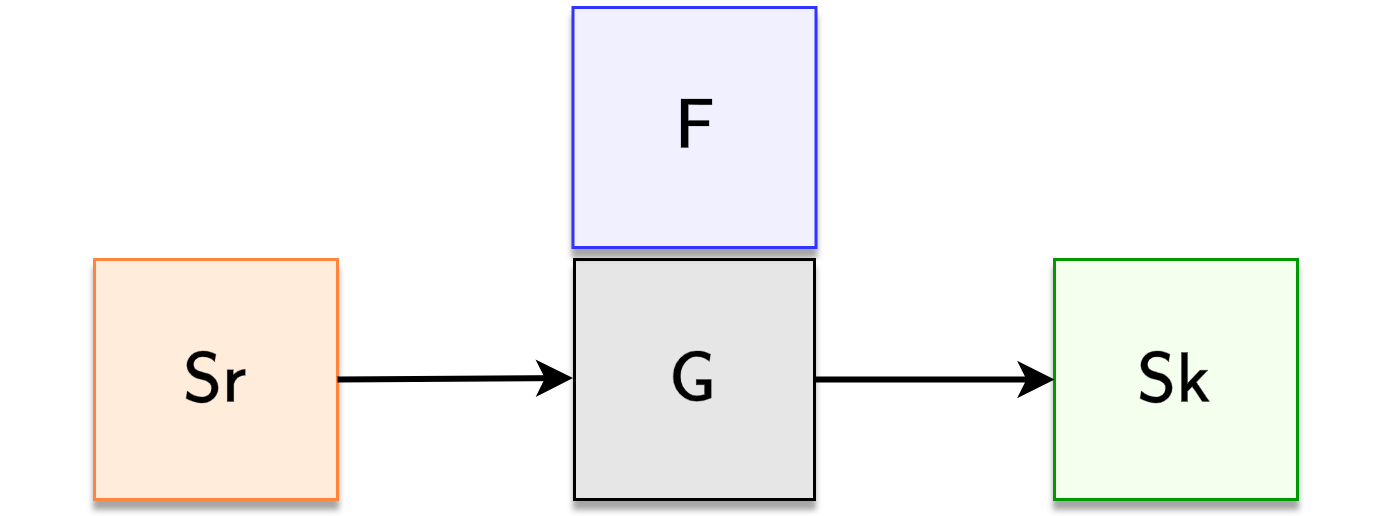
\includegraphics[scale = 0.7]{images/3-Engine/DP-Stages-1.png}
  \caption{Initial configuration of a Dynamic Pipeline. An initial $\mathsf{DP}$ consists of three stages: \emph{Source} ($\mathsf{Sr}$), \emph{Generator} ($\mathsf{G}$) and \emph{Sink} ($\mathsf{Sk}$). Above the  \emph{Generator} ($\mathsf{G}$) the \emph{Filter} ($\mathsf{F}$) parameter. The stages are connected through its channels, represented with the black right arrows.}
  \label{img:DP-Stages-1}
\end{figure}

These stages can be of four different types: \emph{Source} ($\mathsf{Sr}$), \emph{Filter} ($\mathsf{F}$), \emph{Generator} ($\mathsf{G}$) and \emph{Sink} ($\mathsf{Sk}$). \emph{Source} stage are the responsible of obtaining the input data stream and feeding it into the pipeline. \emph{Filter} stages maintain a state and process the incoming data processing it accordingly and/or passing it again to the pipeline. \emph{Generator} stage is in charge of spawning new \emph{Filter} stages when needed based on the incoming data, providing the \textit{dynamic} behavior to the model. Finally, \emph{Sink} stage receives the results, processing and acting on them as needed.
Figure \ref{img:DP-Stages-1} represents the initial configuration of a $\mathsf{DP}$ and Figure \ref{img:DP-Stages-2} depicts the stages of the $\mathsf{DP}$ after a possible evolution, where the \emph{Generator} has created two \emph{Filter} stage instances.\\

\begin{figure}[H]
  \centering
  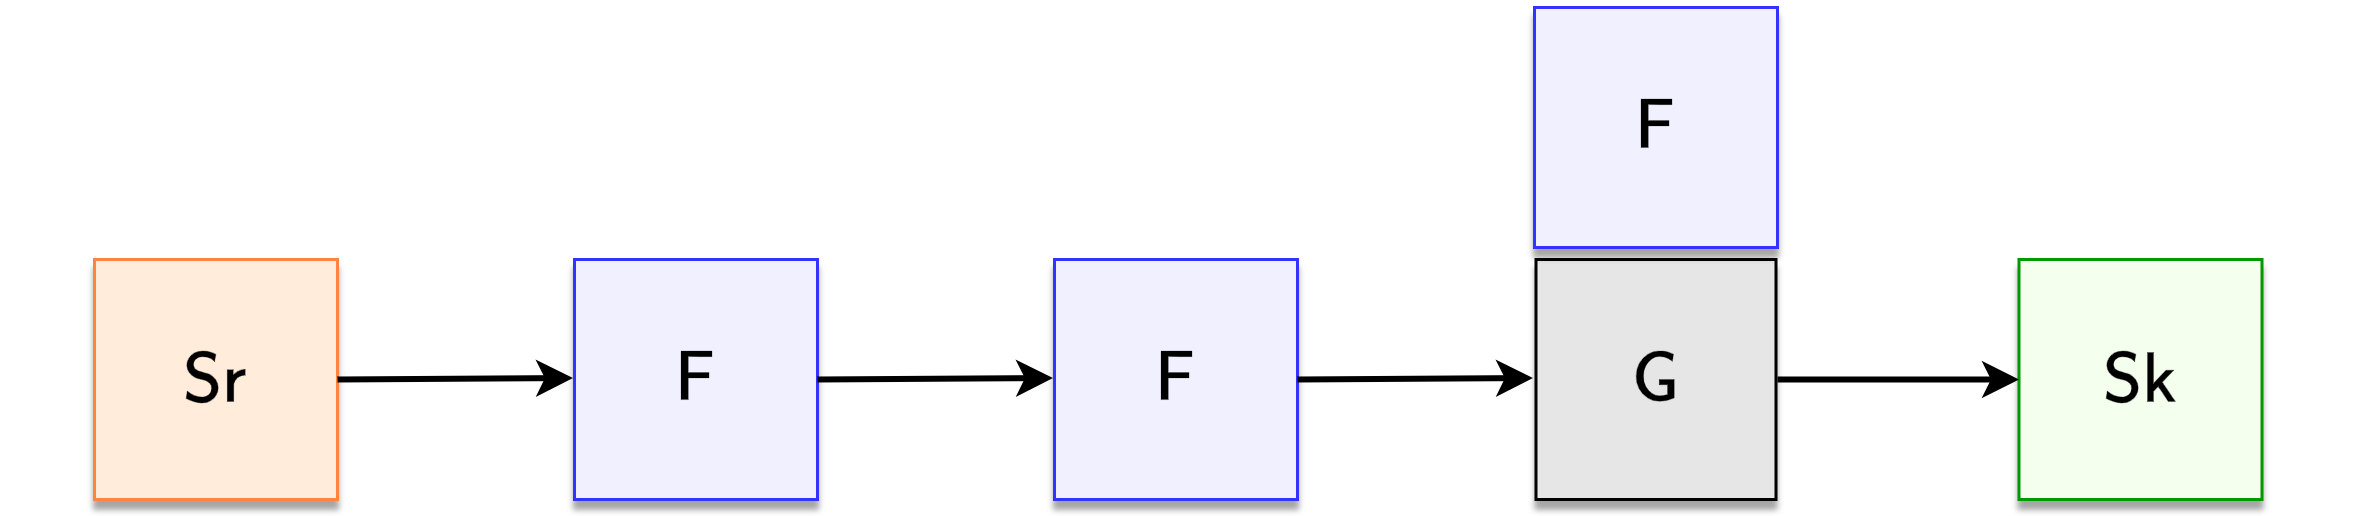
\includegraphics[scale = 0.7]{images/3-Engine/DP-Stages-2.png}
  \caption{Evolution of a $\mathsf{DP}$. After the creation of two \emph{Filter} $\mathsf{F}$ stage instances of the \emph{Filter} parameter (above the $\mathsf{G}$ stage) by the \emph{Generator} $\mathsf{G}$ stage.}
  \label{img:DP-Stages-2}
\end{figure}

The $\mathsf{DPA}$ has been used to model many different problems. In \cite{DP-bitriangles2021} they successfully solved the problem of progressively identify and enumerate bitriangles (i.e. a specific graph pattern) in bipartite evolving graphs. In \cite{DP-Lugosi_Enes_2019} $\mathsf{DPA}$ is used to model the problem of multidimensional range queries, that is, selection queries on objects in a k-dimensional space. Finally, in \cite{DP-Benedi_Garcia_2024} an algorithm to solve the problem of computing and maintaining in practice the minimum spanning tree of dynamic graphs 
using the $\mathsf{DPA}$ is proposed and tested experimentally.\\

In our case, we envision here the architecture of a continuous query engine, the \DPATM, to detect anomalous ATM transactions under the $\mathsf{DPA}$, 
where the continuous input data stream is the stream of the bank ATM transactions, 
and the activity of a Card is tracked using the \emph{Filter} stages of the $\mathsf{DP}$ (see Figure~\ref{img:DP-Stages-2}).
%%
%%
\subsection{Metrics}\label{exps:evaluation-metrics}

The \DPATM\ is an intended to be real-time system for the detection of card-ATM anomalous interactions. As such its evaluation must capture classical metrics such as: mean response time of an answer/detection to be produced, throughput in terms of answers emitted per unit of time, the execution time to process a full stream. 
Additionally, we include other kinds of metrics to quantify and evaluate the efficiency of the system over a certain time period, the so-called \emph{diefficiency} metrics, introduced in \cite{exps-diefficiency}. Unlike the classical metrics, these metrics allow us to have a more complete picture on how the system is behaving during a given period of time, and not just a reduced final picture, by evaluating the progressive emission of results in that time period.

% Describo las métricas una a una en un listado
\begin{itemize}
    \item \textbf{Number of results: \texttt{checks} and \texttt{alerts} produced\\}
    Counters of the number of results that the system produces. Results can be either be counted only as alerts (positive fraud patterns), as fraud pattern checks, both positive (alerts) and negative, or as both at the same time, depending on the experiment. 
    \item \textbf{Response Time (\texttt{RT}) and Mean Response Time (\texttt{MRT})\\}
    \texttt{RT} captures the time it takes for the system to emit a result. It is the elapsed time from the moment a transaction interaction arrives to the system until the result of its respective fraud pattern check is produced. The \texttt{MRT} is the average response time metric for all the results emitted by the system. In a real-time system like ours we are interested in low values of these metrics.
    \item \textbf{Execution Time (\texttt{ET})\\}
    It measures the total time (in seconds) that it takes for the system to consume/process a full input stream. The lower, the better.
    \item \textbf{Throughput (\texttt{T})\\}
    It measures the number of results emitted per time unit. It is calculated as number of results divided by \texttt{ET}. The higher the throughput the better in relation to the performance of our system.
    \item \textbf{Interactions per second (\texttt{interactions/s})\\}
    It measures the number of interactions that the system is able to process per time unit. It is calculated as the total number of interactions that arrived to the system divided by \texttt{ET}. The higher the value of the interactions per second the better in relation to the performance of our system.
    \item \textbf{Time to produce the First Tuple (\texttt{TFFT})\\}
    It is the time required by the system to produce/emit the first result. The lower the value of this metric, the better. Meaning that the system is able to start up fast.
    \item \textbf{\texttt{dief@t} and \texttt{dief@k} metrics\\}
    They measure the \emph{diefficiency} - the continuous efficiency of an engine over a certain time period in terms of the emission of results - and, as mentioned, they allow us to have a more complete picture on how the system is behaving during a given period of time, and not just a reduced final picture. \texttt{dief@t} measures the diefficiency of the engine while producing results in the first \emph{t} time units of execution time. The higher the value of the \texttt{dief@t} metric, the better the continuous behavior. \texttt{dief@k} metric measures the diefficiency of the engine while producing the first \emph{k} results, after the first result is produced. The lower the value of the \texttt{dief@k} metric, the better the continuous behavior.

    \item \textbf{Answer trace\\}
    We provide a similar definition as the one in \cite{exps-diefficiency}. An answer trace can be formally defined as a sequence of pairs $(t_1,r_1),...,(t_n,r_n)$, where $r_i$ is the $ith$ result produced by the engine and $t_i$ is the timestamp that indicates the point in time when $r_i$ is produced. We will record an answer trace for each of the experimental evaluations of the engine, since they provide valuable insights about the continuous efficiency - diefficiency.

\end{itemize}

To obtain the \texttt{dief@t} and \texttt{dief@k} metrics we used the \texttt{diefpy} tool \cite{exps-diefpy-tool}, which calculates them from the generated answer traces by our system. This tool provides us with other utilities for the visualization of the metrics on the obtained sets of results such as: the visualization of answer traces, the generation of radar plots to compare the \texttt{dief@t} with the other conventional/classical metrics, the generation of radar plots to compare the \texttt{dief@k} at different answer completeness percentages, among others.

We additionally extended and modified the tool for our specific needs. This was done in order to visualize other metrics, especially the \MRT, but also others like the throughput \texttt{T}, \texttt{interactions/s} or the \texttt{TFFT}.